\documentclass[11pt,a4paper]{article}
\usepackage[paperwidth=13.333in,paperheight=7.5in,margin=0pt]{geometry}

\usepackage[utf8]{inputenc}
\usepackage[T1]{fontenc}
\usepackage{lmodern}
\usepackage{amsmath,amssymb,amsfonts,bm}
\usepackage{graphicx}
\graphicspath{{../img/}{./img/}{img/}}
\usepackage{xcolor}
\usepackage{tikz}
\usetikzlibrary{calc,shapes.geometric,positioning}
\usepackage{booktabs}
\usepackage{array}
\usepackage{hyperref}

% Color Palette
\definecolor{navy}{HTML}{002060}
\definecolor{primaryblue}{HTML}{184C78}
\definecolor{accent}{HTML}{2980B9}
\definecolor{darkgray}{HTML}{2C3E50}
\definecolor{lightbg}{HTML}{F5F7FA}
\definecolor{bordergray}{HTML}{C8CDD2}
\definecolor{mutedgray}{HTML}{7F8C8D}
\definecolor{crimson}{HTML}{9E1636}
\definecolor{successgreen}{HTML}{27AE60}
\definecolor{gold}{HTML}{B48C14}

\pagestyle{empty}
\setlength{\parindent}{0pt}

% Total number of slides
\newcommand{\totalslides}{13}

% Helper: Place text block at (x, y) inches from top-left with width w inches
\newcommand{\at}[4]{%
  \node[anchor=north west,inner sep=0pt,text width=#3in,align=left]
    at ([xshift=#1in,yshift=-#2in]current page.north west) {#4};%
}

% Per-slide line spacing
\newcommand{\slidespread}[1]{\linespread{#1}\selectfont}
\newcommand{\fs}[2]{\fontsize{#1pt}{#2pt}\selectfont}

% Slide Header Macro
\newcommand{\slideheader}[3]{%
  % Top-left KU Logo
  \node[anchor=west,inner sep=0pt]
    at ([xshift=0.50in,yshift=-0.70in]current page.north west)
    {
\includegraphics[width=0.70in,height=0.82in]{ku_logo.png}};
  % Vertical accent bar
  \fill[accent] ([xshift=1.35in,yshift=-0.25in]current page.north west)
    rectangle ++(0.06in,-0.90in);
  % Title & Subtitle Node
  \node[anchor=west,inner sep=0pt,text width=11.2in,align=left]
    at ([xshift=1.55in,yshift=-0.70in]current page.north west) {%
      {\fs{11}{13}\bfseries\color{accent}\MakeUppercase{#1}\quad|\quad}%
      {\fs{20.5}{24}\bfseries\color{navy}#2}\\[0.18em]
      \if\relax\detokenize{#3}\relax\else{\fs{13}{16}\color{darkgray}#3}\fi
    };
}

% Slide Footer Macro
\newcommand{\slidefooter}[1]{%
  \fill[bordergray] ([xshift=0.5in,yshift=-7.0in]current page.north west)
    rectangle ++(12.333in,-0.02in);
  \at{0.5}{7.06}{2.5}{\fs{10}{12}\color{mutedgray}November 19, 2026}
  \node[anchor=north,inner sep=0pt]
    at ([yshift=-7.06in]current page.north)
    {\fs{10}{12}\color{mutedgray}Chong Shik Park, Ph.D. \enspace$|$\enspace Korea University, Sejong \enspace$|$\enspace Mini-Hackathon Session};
  \node[anchor=north east,inner sep=0pt]
    at ([xshift=-0.5in,yshift=-7.06in]current page.north east)
    {\fs{10}{12}\bfseries\color{primaryblue}#1 / \totalslides};
}

% Standard Content Card Macro
\newcommand{\drawcard}[5]{%
  \draw[rounded corners=8pt,fill=lightbg,draw=bordergray,line width=1.2pt]
    ([xshift=#1in,yshift=-#2in]current page.north west)
    rectangle ++(#3in,-#4in);
  \if\relax\detokenize{#5}\relax\else
    \pgfmathsetmacro{\cx}{#1+0.25}%
    \pgfmathsetmacro{\cy}{#2+0.22}%
    \pgfmathsetmacro{\cw}{#3-0.5}%
    \at{\cx}{\cy}{\cw}{\fs{15.5}{19}\bfseries\color{navy}#5}
  \fi
}

% Code Box Helper Macro
\newcommand{\drawcodecard}[4]{%
  \draw[rounded corners=4pt,fill=white,draw=bordergray,line width=0.9pt]
    ([xshift=#1in,yshift=-#2in]current page.north west)
    rectangle ++(#3in,-#4in);
}

\begin{document}
\linespread{1.22}\selectfont

% ==============================================================================
% SLIDE 1: Title Slide
% ==============================================================================
\begin{tikzpicture}[remember picture,overlay]
  \slidespread{1.22}
  \draw[rounded corners=10pt,fill=white,draw=primaryblue,line width=2pt]
    ([xshift=0.5in,yshift=-0.5in]current page.north west) rectangle ++(12.333in,-6.5in);
  \fill[accent] ([xshift=0.5in,yshift=-0.5in]current page.north west)
    rectangle ++(12.333in,-0.1in);

  \node[anchor=north west,inner sep=0pt]
    at ([xshift=1.0in,yshift=-0.85in]current page.north west)
    {
\includegraphics[width=0.81in,height=0.95in]{ku_logo.png}};

  \at{2.05}{0.92}{10.2}{\fs{13}{16}\bfseries\color{primaryblue}%
    AI Applications in Accelerators Tutorial \& Mini-Hackathon\\[0.15em]
    {\fs{11}{14}\color{mutedgray}Department of Accelerator Science $\cdot$ Center for Accelerator Research $\cdot$ Korea University, Sejong}
  }

  \fill[bordergray] ([xshift=1.0in,yshift=-2.0in]current page.north west)
    rectangle ++(11.333in,-0.02in);

  \at{1.0}{2.25}{11.333}{%
    {\fs{26}{30}\bfseries\color{navy}Session 2: Beam Orbit Alignment Mini-Hackathon}\\[0.45em]
    {\fs{15}{19}\color{accent}Closed-Loop Neural Surrogates, Reinforcement Learning, and Bayesian Optimization}
  }

  \drawcard{1.0}{3.3}{11.333}{2.2}{}
  \at{1.3}{3.55}{10.7}{\fs{13.5}{19}\color{darkgray}%
    {\bfseries\color{navy}Challenge Objective:}\enspace Stabilize an unknown distorted beam orbit in a non-linear 15-meter transport line to sub-30 $\mu\text{m}$ RMS precision within a 50-step budget, using constrained magnetic actuators under cubic core saturation.\\[0.5em]
    {\bfseries\color{navy}Unified Benchmark:}\enspace Participants develop and evaluate four competitor controllers simultaneously (\textbf{Baseline 0}, \textbf{Baseline 1}, \textbf{Track 2}, and \textbf{Track 3}) across 30 standardized seeds with live Weights \& Biases leaderboard telemetry.
  }

  \at{1.0}{5.75}{11.333}{\fs{12.5}{16}\color{darkgray}%
    \textbf{Organizer \& Session Lead:}\enspace Chong Shik Park, Ph.D. \quad$|$\quad Korea University, Sejong\\[0.2em]
    \textbf{Date \& Venue:}\enspace November 19, 2026 \quad$|$\quad Hands-on Computational Session (13:30 -- 17:00 KST)
  }

  \fill[primaryblue] ([xshift=0.5in,yshift=-6.95in]current page.north west)
    rectangle ++(12.333in,-0.05in);
\end{tikzpicture}\clearpage

% ==============================================================================
% SLIDE 2: Afternoon Schedule & Milestones
% ==============================================================================
\begin{tikzpicture}[remember picture,overlay]
  \slidespread{1.24}
  \slideheader{Schedule \& Roadmap}{Afternoon Mini-Hackathon Timeline (13:30 -- 17:00)}{Open hands-on optimization: participants can run and iterate on all tracks simultaneously}

  \drawcard{0.8}{1.4}{11.733}{5.3}{Mini-Hackathon Operational Milestones}

  \at{1.1}{2.15}{11.1}{\fs{12}{17.5}\color{darkgray}%
    \begin{tabular}{p{2.1in}p{2.8in}p{5.8in}}
      \toprule
      \textbf{Time Window} & \textbf{Session Milestone} & \textbf{Operational Focus \& Hands-on Activities} \\
      \midrule
      {\bfseries\color{primaryblue}13:30 -- 13:45 (15 min)} & {\bfseries Environment \& Setup} & Unpack offline bundle, launch Docker container via launcher scripts, open participant notebook, set \texttt{TEAM\_NAME}, and verify Baseline 0 reference. \\
      \addlinespace[0.9em]
      {\bfseries\color{primaryblue}13:45 -- 16:15 (2.5 hrs)} & {\bfseries Multi-Track Optimization (Open Hackathon)} & \textbf{Open development window:} participants develop, tune, and benchmark all tracks concurrently without sequential restrictions (surrogate, RL, BO, and callbacks). \\
      \addlinespace[0.9em]
      {\bfseries\color{primaryblue}16:15 -- 16:30 (15 min)} & {\bfseries Final Submission \& Score Freeze} & Execute final 30-seed benchmark in Step 5, confirm telemetry on live W\&B leaderboard, and inspect trajectory alignment plots. \\
      \addlinespace[0.9em]
      {\bfseries\color{gold}16:30 -- 17:00 (30 min)} & {\bfseries Showcase \& Awards Ceremony} & 3-minute lightning presentations per team, live leaderboard review, and presentation of hackathon champion awards. \\
      \bottomrule
    \end{tabular}
  }

  \slidefooter{2}
\end{tikzpicture}\clearpage

% ==============================================================================
% SLIDE 3: Environment & Setup (Offline Bundle & Container Execution)
% ==============================================================================
\begin{tikzpicture}[remember picture,overlay]
  \slidespread{1.22}
  \slideheader{Environment \& Setup}{Offline Bundle Structure \& Container Execution}{Zero-dependency offline distribution, one-click platform launchers, and container workspace}

  % Left Card: Bundle Structure
  \drawcard{0.8}{1.4}{5.7}{5.3}{Offline Distribution Package Structure}
  \at{1.05}{2.02}{5.2}{\fs{11.5}{15}\color{darkgray}%
    {\bfseries\color{navy}100\% Self-Contained Offline Bundle (\texttt{ai4acc-hackathon.zip}):}\\[0.15em]
    Everything required to run the hackathon is pre-packaged locally:
  }
  \drawcodecard{1.05}{2.62}{5.2}{1.60}
  \at{1.2}{2.76}{4.9}{\fs{9}{12}\ttfamily\color{darkgray}%
    ai4acc-hackathon/\\
    \ \ \mbox{}|-- ai4acc-image.tar.gz\ \ \ \ \ \ \ \# Docker image (\~{}400 MB)\\
    \ \ \mbox{}|-- run\_hackathon\_windows.bat \# Windows launcher\\
    \ \ \mbox{}|-- run\_hackathon\_mac\_linux.sh\# macOS/Linux launcher\\
    \ \ \mbox{}|-- wandb.apikey\ \ \ \ \ \ \ \ \ \ \ \ \ \# Shared W\&B key\\
    \ \ \mbox{}|-- image-id.txt\ \ \ \ \ \ \ \ \ \ \ \ \ \# Image cache hash\\
    \ \ \mbox{}`-- README.txt\ \ \ \ \ \ \ \ \ \ \ \ \ \ \ \# Offline instructions
  }
  \at{1.05}{4.40}{5.2}{\fs{11}{15}\color{darkgray}%
    {\bfseries\color{navy}$\bullet$ Zero-Dependency Execution:}\enspace Operates completely offline without internet or Wi-Fi dependencies during the workshop.\\[0.35em]
    {\bfseries\color{navy}$\bullet$ Pre-Configured Telemetry:}\enspace The launcher automatically injects \texttt{wandb.apikey} as \texttt{WANDB\_API\_KEY} for live leaderboard sync.\\[0.35em]
    {\bfseries\color{navy}$\bullet$ Pre-Loaded Environment:}\enspace Contains Python 3.12, Gymnasium, PyTorch, scikit-learn, JupyterLab, and the simulation harness.
  }

  % Right Card: How to Run Docker
  \drawcard{6.8}{1.4}{5.7}{5.3}{How to Launch Docker \& JupyterLab}
  \at{7.05}{2.02}{5.2}{\fs{11.5}{15}\color{darkgray}%
    {\bfseries\color{navy}Step 1: Ensure Docker Desktop is Running}\\[0.15em]
    Verify Docker Desktop is active (whale icon in system tray).
  }
  \drawcodecard{7.05}{2.62}{5.2}{1.60}
  \at{7.2}{2.76}{4.9}{\fs{9}{12}\ttfamily\color{darkgray}%
    \# Windows: Double-click launcher\\
    run\_hackathon\_windows.bat\\[0.3em]
    \# macOS / Linux (in terminal):\\
    ./run\_hackathon\_mac\_linux.sh\\[0.3em]
    \# Browser opens automatically: http://localhost:8888/lab
  }
  \at{7.05}{4.40}{5.2}{\fs{11}{15}\color{darkgray}%
    {\bfseries\color{navy}$\bullet$ Step 2: Instant Browser Access:}\enspace JupyterLab opens automatically in your browser. Token authentication is disabled for instant entry.\\[0.35em]
    {\bfseries\color{navy}$\bullet$ Step 3: Open Participant Notebook:}\enspace In the Jupyter tree, open \texttt{notebooks/Single\_Notebook\_Beam\_Orbit\_Predictor\_Participant.ipynb}.\\[0.35em]
    {\bfseries\color{primaryblue}$\bigstar$ Step 4: Configure Team Name:}\enspace Set your team name in Step 0: \texttt{TEAM\_NAME = "Team\_Alpha"} before running Baseline 0!
  }

  \slidefooter{3}
\end{tikzpicture}\clearpage

% ==============================================================================
% SLIDE 4: Physical System & Beamline Layout
% ==============================================================================
\begin{tikzpicture}[remember picture,overlay]
  \slidespread{1.24}
  \slideheader{Beamline Physics}{Lattice Architecture \& Diagnostic Instrumentation}{A 15-meter transport line balancing focusing optics, dipole steering, and sub-micron diagnostics}

  \drawcard{0.8}{1.4}{5.7}{5.3}{Magnetic Lattice \& Diagnostic Geometry}
  \at{1.05}{2.1}{5.2}{\fs{12.5}{17}\color{darkgray}%
    {\bfseries\color{navy}$\bullet$ Section Length \& Optics:}\\[0.2em]
    $15.0\text{ m}$ single-pass transport section with alternating focusing (\texttt{QF}) and defocusing (\texttt{QD}) quadrupoles shaping betatron phase advance $\psi(s)$.\\[0.6em]
    {\bfseries\color{navy}$\bullet$ 6 Dipole Steering Correctors:}\\[0.2em]
    3 Horizontal (\texttt{HCM1-3}) and 3 Vertical (\texttt{VCM1-3}) magnets located at $s \in [0.2, 8.0]\text{ m}$. Total current bounds $[-5.0, +5.0]\text{ A}$.\\[0.6em]
    {\bfseries\color{navy}$\bullet$ 12 Beam Position Monitors (BPMs):}\\[0.2em]
    Diagnostic stations at $s \in [1.0, 15.0]\text{ m}$ measuring transverse beam centroid displacement $\mathbf{Y} \in \mathbb{R}^{12}$ in millimeters ($mm$).\\[0.6em]
    {\bfseries\color{navy}$\bullet$ Actuator Hardware Constraint:}\\[0.2em]
    Per-step adjustment is strictly bounded: $\Delta \mathbf{I} \in [-0.8, +0.8]\text{ A}$.
  }

  \drawcard{6.8}{1.4}{5.7}{5.3}{Core Beamline Schematic Diagram}
  \at{7.05}{2.1}{5.2}{\fs{12.5}{17}\color{darkgray}%
    \centering
    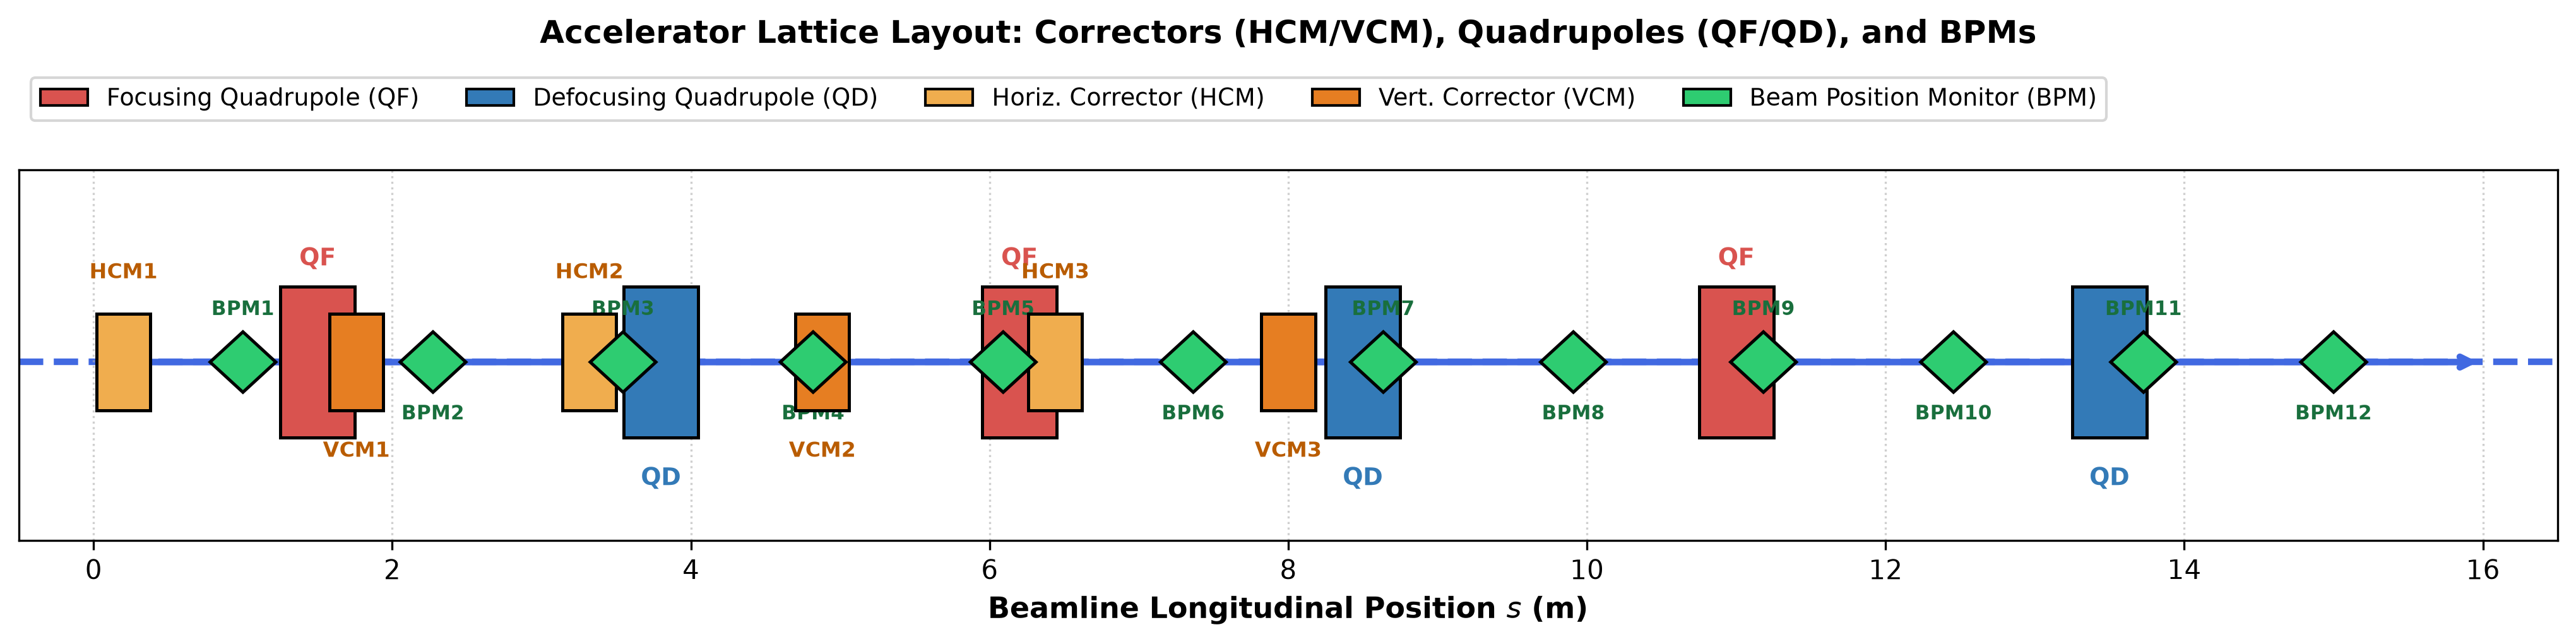
\includegraphics[width=5.1in,height=2.3in,keepaspectratio]{beamline.png}\\[0.5em]
    \raggedright
    {\bfseries\color{navy}$\bullet$ Single-Pass Causality:}\enspace Steerers only deflect the orbit at downstream BPMs ($s_j > s_i$). Upstream stations remain unaffected ($R_{ij} = 0$).\\[0.4em]
    {\bfseries\color{navy}$\bullet$ Transport-Line Response Matrix:}\\[0.2em]
    $R_{ij} = \frac{1.2 \sin(2\pi \cdot 0.18 (s_j - s_i))}{1 + 0.05 (s_j - s_i)}$ for $s_j > s_i$, modeling betatron oscillation with slowly decaying amplitude envelope.
  }

  \slidefooter{4}
\end{tikzpicture}\clearpage

% ==============================================================================
% SLIDE 5: Physical Response & Non-Linear Saturation
% ==============================================================================
\begin{tikzpicture}[remember picture,overlay]
  \slidespread{1.26}
  \slideheader{Physics Response Model}{Cubic Core Saturation \& Initial 6-Kick Distortion}{Mathematical formulation of the forward simulation environment and sensor noise floor}

  \drawcard{0.8}{1.4}{5.7}{5.3}{Forward Physical Orbit Model}
  \at{1.05}{2.1}{5.2}{\fs{13}{18}\color{darkgray}%
    {\bfseries\color{navy}$\bullet$ Response Equation with Saturation:}\\[0.3em]
    $\mathbf{Y} = \mathbf{I}\mathbf{R} - 0.015\,(\mathbf{I}^3 \mathbf{R}) + \mathbf{Y}_0 + \boldsymbol{\epsilon}$\\[0.5em]
    where $\mathbf{I} \in \mathbb{R}^6$ is total corrector current, $\mathbf{R} \in \mathbb{R}^{6 \times 12}$ is the linear response, and $\boldsymbol{\epsilon} \sim \mathcal{N}(0, 0.010^2)$ is Gaussian sensor noise.\\[0.6em]
    {\bfseries\color{navy}$\bullet$ Non-Linear Core Saturation:}\\[0.2em]
    The odd-symmetric cubic term $-0.015 \mathbf{I}^3 \mathbf{R}$ models iron-core permeability degradation while preserving field polarity $B(-I) = -B(I)$.\\[0.6em]
    {\bfseries\color{crimson}$\bullet$ Loss of Actuator Authority:}\\[0.2em]
    At $|I| = 2.5\text{ A}$, saturation reduces steering response by $\approx 23\%$. Linear controllers overshoot or chatter.
  }

  \drawcard{6.8}{1.4}{5.7}{5.3}{Initial Distortion \& Actuator Budget}
  \at{7.05}{2.1}{5.2}{\fs{13}{18}\color{darkgray}%
    {\bfseries\color{navy}$\bullet$ Unknown 6-Kick Error $\mathbf{Y}_0$:}\\[0.3em]
    $\mathbf{Y}_0 = \mathbf{a}\mathbf{R}, \quad a_k \sim \mathcal{U}(-2.5, 2.5)\text{ A}$\\[0.3em]
    Unknown kicks applied at all 6 corrector locations upon reset. Initial orbit error spans $0.93$ to $3.59\text{ mm}$ RMS (mean $1.97\text{ mm}$).\\[0.6em]
    {\bfseries\color{navy}$\bullet$ Exact Cancelling Current:}\\[0.2em]
    Full cancellation requires total currents up to $2.84\text{ A}$, pushing magnets deep into non-linear saturation.\\[0.6em]
    {\bfseries\color{navy}$\bullet$ Minimum Theoretical Step Count:}\\[0.2em]
    With the $|\Delta I| \le 0.8\text{ A}$ hardware slew rate limit, most seeds strictly require at least \textbf{3 to 4 sequential control steps}.
  }

  \slidefooter{5}
\end{tikzpicture}\clearpage

% ==============================================================================
% SLIDE 6: Gymnasium Environment & Agent Contract (FIXED LAYOUT)
% ==============================================================================
\begin{tikzpicture}[remember picture,overlay]
  \slidespread{1.26}
  \slideheader{Gymnasium Interface}{Environment Contract \& Competitor Agent Interface}{Standardized API governing observation space, actions, terminations, and step execution}

  \drawcard{0.8}{1.4}{5.7}{5.3}{Gymnasium Environment Contract}
  \at{1.05}{2.1}{5.2}{\fs{12.5}{17}\color{darkgray}%
    {\bfseries\color{navy}$\bullet$ Observation Space:}\enspace $\mathbf{Y} \in \mathbb{R}^{12}$ (12 BPM centroid readings in $mm$, unclipped).\\[0.5em]
    {\bfseries\color{navy}$\bullet$ Action Space:}\enspace $\Delta\mathbf{I} \in [-0.8, +0.8]^6\text{ A}$ (incremental corrector adjustments).\\[0.5em]
    {\bfseries\color{navy}$\bullet$ State Accumulator:}\enspace $\mathbf{I}_{t+1} = \text{clip}(\mathbf{I}_t + \Delta\mathbf{I}, -5.0, 5.0)\text{ A}$.\\[0.5em]
    {\bfseries\color{navy}$\bullet$ Termination Criterion (\texttt{terminated}):}\\[0.2em]
    Triggered when $\text{RMS} < 0.030\text{ mm}$ ($30\ \mu\text{m}$). Episode succeeds (\texttt{is\_success = True}).\\[0.5em]
    {\bfseries\color{navy}$\bullet$ Truncation Criterion (\texttt{truncated}):}\\[0.2em]
    Triggered if step count reaches $\text{max\_steps} = 50$ without reaching target tolerance. Episode fails.
  }

  \drawcard{6.8}{1.4}{5.7}{5.3}{Standard Competitor Controller Interface}
  % Top introductory text
  \at{7.05}{2.1}{5.2}{\fs{12}{16}\color{darkgray}%
    {\bfseries\color{navy}Universal Agent Execution Contract:}\\[0.2em]
    All competitor controllers implement the standardized \texttt{act} method:
  }
  % Code Box
  \drawcodecard{7.05}{2.7}{5.2}{2.3}
  \at{7.2}{2.85}{4.9}{\fs{9.5}{12.5}\ttfamily\color{darkgray}%
    class BenchmarkController:\\
    \quad def act(self, obs: np.ndarray,\\
    \qquad\qquad\quad info: Optional[dict] = None) -> np.ndarray:\\
    \qquad """\\
    \qquad obs:\quad (12,) BPM readings in mm\\
    \qquad info:\quad \{'rms', 'step', 'currents', ...\}\\
    \qquad Returns:\quad (6,) delta\_I in [-0.8, 0.8] A\\
    \qquad """\\
    \qquad return action
  }
  % Bottom text placed strictly below code card
  \at{7.05}{5.25}{5.2}{\fs{12}{16.5}\color{darkgray}%
    {\bfseries\color{navy}$\bullet$ Total Current Access:}\enspace \texttt{info["currents"]} provides present magnet currents $\mathbf{I}_t$ to compute cubic saturation offsets.\\[0.3em]
    {\bfseries\color{navy}$\bullet$ Output Bounds:}\enspace Actions exceeding $[-0.8, 0.8]\text{ A}$ are hard-clipped by the environment.
  }

  \slidefooter{6}
\end{tikzpicture}\clearpage

% ==============================================================================
% SLIDE 7: The Four Benchmark Controllers
% ==============================================================================
\begin{tikzpicture}[remember picture,overlay]
  \slidespread{1.24}
  \slideheader{Benchmark Controllers}{The Four Competitor Control Paradigms}{From classical pseudo-inverse baseline to neural surrogates, RL policies, and Bayesian optimization}

  \drawcard{0.8}{1.4}{11.733}{5.3}{Comparative Controller Specifications}
  \at{1.1}{2.1}{11.1}{\fs{12}{16.5}\color{darkgray}%
    \begin{tabular}{p{1.9in}p{2.3in}p{4.2in}p{1.9in}}
      \toprule
      \textbf{Controller Track} & \textbf{Algorithmic Law} & \textbf{Mechanism \& Optimization} & \textbf{Benchmark Score} \\
      \midrule
      {\bfseries Baseline 0}\newline Classical Linear SVD & $\Delta\mathbf{I} = -\alpha (\mathbf{R}^T)^\dagger \mathbf{Y}$ & Moore-Penrose pseudo-inverse with fixed gain $\alpha=0.45$. Ignores saturation; oscillates at high gains. & \textbf{635.277 pts}\newline(9.4 steps, 100\% succ) \\
      \addlinespace[0.5em]
      {\bfseries Baseline 1 / Track 1}\newline Supervised Surrogate & $\min_{\Delta\mathbf{I}} \|\mathbf{Y} - f_\theta(\mathbf{I}) + f_\theta(\mathbf{I}+\Delta\mathbf{I})\|^2$ & Trains MLP digital twin $\hat{\mathbf{Y}} = f_\theta(\mathbf{I})$ on offline shots; per-step SciPy \texttt{L-BFGS-B} bounded inversion. & \textbf{779.169 pts}\newline(Tuned: \textbf{924.192 pts}) \\
      \addlinespace[0.5em]
      {\bfseries Track 2}\newline Closed-Loop Policy RL & $\Delta\mathbf{I} = d(t)\,[-\alpha (\mathbf{R}^T)^\dagger \mathbf{Y} + \mathbf{W}\mathbf{Y} + \mathbf{b}]$ & Physics-informed prior + learned residual with dynamic damping schedule $d(t) = 1/(1+\gamma t)$. & \textbf{590.559 pts}\newline(Tuned: \textbf{939.981 pts}) \\
      \addlinespace[0.5em]
      {\bfseries Track 3}\newline Bayesian Optimization & $\min_{\Delta\mathbf{I}} \mu_{\text{GP}}(\Delta\mathbf{I}) - \kappa \sigma_{\text{GP}} + \lambda \|\Delta\mathbf{I}\|^2$ & GaussianProcessRegressor (Mat\'{e}rn-5/2) with Lower Confidence Bound (LCB) under epistemic uncertainty. & \textbf{878.384 pts}\newline(Tuned: \textbf{909.942 pts}) \\
      \bottomrule
    \end{tabular}
  }

  \slidefooter{7}
\end{tikzpicture}\clearpage

% ==============================================================================
% SLIDE 8: Official Scoring Formula
% ==============================================================================
\begin{tikzpicture}[remember picture,overlay]
  \slidespread{1.26}
  \slideheader{Evaluation \& Scoring}{Official Hackathon Scoring Formula (0 to 1000 Points)}{Balancing robust convergence, rapid iteration speed, and sub-micron landing precision}

  \drawcard{0.8}{1.4}{5.7}{5.3}{Mathematical Scoring Formulation}
  \at{1.05}{2.1}{5.2}{\fs{13}{18}\color{darkgray}%
    {\bfseries\color{navy}$\bullet$ Overall Score:}\enspace $\text{Score} = \frac{1}{30}\sum_{k=1}^{30} s_k$\\[0.4em]
    Evaluated strictly across \textbf{30 standardized seeds} (\texttt{seeds = range(1, 31)}).\\[0.6em]
    {\bfseries\color{navy}$\bullet$ Per-Seed Score $s_k$ Breakdown:}\\[0.3em]
    $s_k = 0$ if seed fails ($\ge 50$ steps or $\text{RMS} \ge 0.03\text{ mm}$).\\[0.4em]
    If seed succeeds ($n_k$ steps, final $\text{RMS}_k$):
    \begin{equation*}
      s_k = \underbrace{400}_{\text{Success}} + \underbrace{300 \max\!\left(0, \frac{20 - n_k}{19}\right)}_{\text{Speed (1 to 20 steps)}} + \underbrace{300 \text{clip}\!\left(\frac{\ln(0.030/\text{RMS}_k)}{\ln(3)}, 0, 1\right)}_{\text{Precision (0.030 to 0.010 mm)}}
    \end{equation*}
  }

  \drawcard{6.8}{1.4}{5.7}{5.3}{Component Analysis \& Strategic Trade-offs}
  \at{7.05}{2.1}{5.2}{\fs{13}{18}\color{darkgray}%
    {\bfseries\color{navy}1. Success Foundation (400 pts):}\\[0.2em]
    Robustness is paramount. A single divergence sets seed score to 0 and costs 33.3 total benchmark points.\\[0.6em]
    {\bfseries\color{navy}2. Speed Component (up to 300 pts):}\\[0.2em]
    Full 300 pts earned at 1 step; decays linearly to 0 at 20 steps. Each saved step earns $\approx 15.8$ points.\\[0.6em]
    {\bfseries\color{navy}3. Precision Component (up to 300 pts):}\\[0.2em]
    Logarithmic bonus rewarding sub-micron alignment. Earns 0 at $0.030\text{ mm}$ boundary, up to 300 pts at $0.010\text{ mm}$ sensor floor ($0.017\text{ mm}$ earns $\approx 150$ pts).\\[0.6em]
    {\bfseries\color{mutedgray}Current Norm:}\enspace Reported but not scored.
  }

  \slidefooter{8}
\end{tikzpicture}\clearpage

% ==============================================================================
% SLIDE 9: Participant Modification Rules
% ==============================================================================
\begin{tikzpicture}[remember picture,overlay]
  \slidespread{1.24}
  \slideheader{Modification Rules}{What Participants CAN and CANNOT Modify}{Clear operational boundary preserving scientific ground truth while maximizing design freedom}

  \drawcard{0.8}{1.4}{5.7}{5.3}{Permitted Participant Modifications [CAN MODIFY]}
  \at{1.05}{2.1}{5.2}{\fs{12.5}{17}\color{darkgray}%
    {\bfseries\color{successgreen}$\checkmark$ TODO 1 (Surrogate Digital Twin):}\\[0.2em]
    MLP hidden layers (e.g. \texttt{(128, 64, 32)}), activation (\texttt{relu}, \texttt{tanh}), solver (\texttt{adam}, \texttt{lbfgs}), training samples ($n=1500 \to 3000$), current bounds $[-3.0, 3.0]\text{ A}$.\\[0.5em]
    {\bfseries\color{successgreen}$\checkmark$ TODO 2 (Track 2 RL Policy Agent):}\\[0.2em]
    Full \texttt{act()} design: starting gain $\alpha_0$, adaptive gain schedules, residual weights $\mathbf{W}$, saturation compensation on $\mathbf{I}_t$, chatter damping.\\[0.5em]
    {\bfseries\color{successgreen}$\checkmark$ TODO 3 (Track 3 Bayesian Optimization):}\\[0.2em]
    GP kernel specification (\texttt{Matern52}, \texttt{WhiteKernel}), calibration shots, acquisition exploration $\kappa$, regularizer $\lambda$.\\[0.5em]
    {\bfseries\color{successgreen}$\checkmark$ Step 4 Callbacks:}\enspace Register \texttt{step\_callback} and \texttt{episode\_callback} for B1, Track 2, and Track 3.
  }

  \drawcard{6.8}{1.4}{5.7}{5.3}{Strict Ground Truth Boundaries [DO NOT MODIFY]}
  \at{7.05}{2.1}{5.2}{\fs{12.5}{17}\color{darkgray}%
    {\bfseries\color{crimson}$\times$ Baseline 0 Reference:}\\[0.2em]
    The \texttt{gain=0.45} and classical SVD formulation must not be altered. Baseline 0 always runs without callbacks.\\[0.5em]
    {\bfseries\color{crimson}$\times$ Physical Simulation Ground Truths:}\\[0.2em]
    Do not modify $\mathbf{R}$, target $\text{RMS} = 0.030\text{ mm}$, $\text{max\_steps} = 50$, cubic saturation factor $0.015$, or noise $\sigma = 0.010\text{ mm}$.\\[0.5em]
    {\bfseries\color{crimson}$\times$ Evaluation Protocol:}\\[0.2em]
    Benchmark evaluation must run on standardized seeds \texttt{range(1, 31)} via the locked Step 5 harness.\\[0.5em]
    {\bfseries\color{crimson}$\times$ Action Hardware Limits:}\\[0.2em]
    Actions must respect $[-0.8, +0.8]\text{ A}$ per step and total magnet current limits $[-5.0, +5.0]\text{ A}$.
  }

  \slidefooter{9}
\end{tikzpicture}\clearpage

% ==============================================================================
% SLIDE 10: Advanced Strategy: Callbacks (FIXED BALANCED LAYOUT)
% ==============================================================================
\begin{tikzpicture}[remember picture,overlay]
  \slidespread{1.22}
  \slideheader{Strategic Tuning}{Online Callbacks \& Adaptive Damping Strategies}{Unlocking 900+ scores via dynamic gain schedules, saturation watchdogs, and meta-tuning}

  % Left Card: Step Callback
  \drawcard{0.8}{1.4}{5.7}{5.3}{Step Callback: Precision Damping \& Watchdogs}
  \at{1.05}{2.02}{5.2}{\fs{11.5}{15}\color{darkgray}%
    {\bfseries\color{navy}Adaptive Near-Target Damping (\texttt{step\_callback}):}\\[0.15em]
    Throttle gain near target to glide into noise floor without overshoot:
  }
  \drawcodecard{1.05}{2.62}{5.2}{1.45}
  \at{1.2}{2.76}{4.9}{\fs{9.5}{13}\ttfamily\color{darkgray}%
    def my\_step\_callback(step\_data, agent):\\
    \quad rms = step\_data["info"]["rms"]\\
    \quad if rms < 0.040 and hasattr(agent, "gain"):\\
    \qquad agent.gain *= 0.94  \# Glide into noise floor!
  }
  \at{1.05}{4.30}{5.2}{\fs{11}{15}\color{darkgray}%
    {\bfseries\color{navy}$\bullet$ Saturation Watchdog:}\enspace If $\|\mathbf{I}_t\|_\infty > 2.5\text{ A}$, scale back action size to prevent cubic non-linear overshoots deep in core saturation.\\[0.35em]
    {\bfseries\color{navy}$\bullet$ Step Telemetry Access:}\enspace \texttt{step\_data} exposes \texttt{"step"}, \texttt{"obs"}, \texttt{"action"}, and \texttt{"info"} (\texttt{"rms"} and total \texttt{"currents"}).\\[0.35em]
    {\bfseries\color{navy}$\bullet$ Implementation:}\enspace Register in \texttt{CALLBACKS["step\_callback"]} in Step 4. See \texttt{docs/CALLBACK\_EXAMPLES.md} for recipes.
  }

  % Right Card: Episode Callback
  \drawcard{6.8}{1.4}{5.7}{5.3}{Episode Callback: Reset \& Meta-Tuning}
  \at{7.05}{2.02}{5.2}{\fs{11.5}{15}\color{darkgray}%
    {\bfseries\color{navy}Per-Seed State Reset (\texttt{episode\_callback}):}\\[0.15em]
    Reset dynamic gain and integrator state back to defaults between seeds:
  }
  \drawcodecard{7.05}{2.62}{5.2}{1.45}
  \at{7.2}{2.76}{4.9}{\fs{9.5}{13}\ttfamily\color{darkgray}%
    def my\_episode\_callback(ep\_data, agent):\\
    \quad if hasattr(agent, "gain"):\\
    \qquad agent.gain = 1.05  \# Restore baseline gain
  }
  \at{7.05}{4.30}{5.2}{\fs{11}{15}\color{darkgray}%
    {\bfseries\color{navy}$\bullet$ Cross-Seed Meta-Tuning (Tournament 3 Winner):}\enspace Adapt base gain across seeds based on prior outcomes: boost speed if prior seed converged in $\le 3$ steps; damp if struggling.\\[0.35em]
    {\bfseries\color{navy}$\bullet$ Episode Telemetry Access:}\enspace \texttt{ep\_data} exposes \texttt{"seed"}, \texttt{"final\_rms"}, \texttt{"steps"}, \texttt{"success"}, and \texttt{"current\_norm"}.\\[0.35em]
    {\bfseries\color{crimson}$\bullet$ Disclosure Rule:}\enspace Any cross-seed state retention must be disclosed during your team's 3-minute lightning presentation!
  }

  \slidefooter{10}
\end{tikzpicture}\clearpage

% ==============================================================================
% SLIDE 11: Zero-Friction W&B Workflow (FIXED LAYOUT)
% ==============================================================================
\begin{tikzpicture}[remember picture,overlay]
  \slidespread{1.26}
  \slideheader{Live Leaderboard}{Zero-Friction Weights \& Biases Workflow}{Automated telemetry streaming, 30-seed breakdown tables, and real-time competition standings}

  % Left Card: Authentication Setup
  \drawcard{0.8}{1.4}{5.7}{5.3}{Zero-Friction Authentication Setup}
  \at{1.05}{2.1}{5.2}{\fs{12.5}{17}\color{darkgray}%
    {\bfseries\color{navy}$\bullet$ No W\&B Account Required:}\\[0.2em]
    The offline distribution bundle contains the shared leaderboard key in \texttt{wandb.apikey}. Launchers pass it automatically.\\[0.5em]
    {\bfseries\color{navy}$\bullet$ Step 0: Set Team Identifier:}\\[0.2em]
    In Step 0 of the notebook, configure your unique team name:
  }
  \drawcodecard{1.05}{3.7}{5.2}{1.0}
  \at{1.2}{3.85}{4.9}{\fs{9.5}{12.5}\ttfamily\color{darkgray}%
    TEAM\_NAME = "Team\_Alpha"\\
    WANDB\_PROJECT = "ai4acc-mini-hackathon-2026"
  }
  \at{1.05}{4.95}{5.2}{\fs{12.5}{17}\color{darkgray}%
    {\bfseries\color{navy}$\bullet$ Seamless Local Fallback:}\\[0.2em]
    If offline or in isolated network environments, the benchmark executes locally and prints complete scorecard tables.
  }

  % Right Card: Leaderboard & Telemetry
  \drawcard{6.8}{1.4}{5.7}{5.3}{Automated Telemetry \& Live Leaderboard}
  \at{7.05}{2.1}{5.2}{\fs{12.5}{17}\color{darkgray}%
    {\bfseries\color{navy}$\bullet$ Step 5 Benchmark Execution:}\\[0.2em]
    Running Step 5 evaluates all 4 controllers across seeds 1--30 simultaneously and streams telemetry to W\&B.\\[0.5em]
    {\bfseries\color{navy}$\bullet$ Tracked Metrics in W\&B:}\\[0.2em]
    \texttt{challenge\_score}, \texttt{score\_success}, \texttt{score\_speed}, \texttt{score\_precision}, \texttt{mean\_steps}, \texttt{mean\_final\_rms\_mm}, \texttt{seed\_breakdown\_table}.\\[0.5em]
    {\bfseries\color{navy}$\bullet$ Central Live Leaderboard URL:}\\[0.2em]
    {\fs{10.5}{14}\color{primaryblue}\texttt{https://wandb.ai/ai4acc-mini-hackathon-2026/\\ai4acc-mini-hackathon-2026}}\\[0.3em]
    Sort by \texttt{challenge\_score} to view live workshop ranks!
  }

  \slidefooter{11}
\end{tikzpicture}\clearpage

% ==============================================================================
% SLIDE 12: Team Lightning Showcase & Awards
% ==============================================================================
\begin{tikzpicture}[remember picture,overlay]
  \slidespread{1.24}
  \slideheader{Showcase \& Awards}{Team Lightning Presentations \& Hackathon Awards (16:30 -- 17:00)}{Celebrating technical excellence, control innovation, and practical beam alignment performance}

  \drawcard{0.8}{1.4}{5.7}{5.3}{3-Minute Lightning Team Presentations}
  \at{1.05}{2.1}{5.2}{\fs{12.5}{17}\color{darkgray}%
    {\bfseries\color{navy}Presentation Format:}\enspace 3 minutes per team directly from your laptop or W\&B run dashboard.\\[0.5em]
    {\bfseries\color{navy}Required Presentation Elements:}\\[0.2em]
    1. {\bfseries Architecture Overview:}\enspace Which track did you focus on? (MLP surrogate, RL policy, or Bayesian Opt?)\\[0.3em]
    2. {\bfseries Strategic Innovations:}\enspace What hyperparameter, damping schedule, or callback gave your biggest score boost?\\[0.3em]
    3. {\bfseries Scorecard Display:}\enspace Display your team's W\&B run URL and trajectory plot (\texttt{img/benchmark\_trajectories.png}).\\[0.3em]
    4. {\bfseries Architectural Disclosure:}\enspace Did your agent use callbacks or cross-seed memory?
  }

  \drawcard{6.8}{1.4}{5.7}{5.3}{Official Hackathon Award Categories}
  \at{7.05}{2.1}{5.2}{\fs{12.5}{17}\color{darkgray}%
    {\bfseries\color{gold}[Grand Champion Award]}\\[0.2em]
    Highest official benchmark score across all 30 seeds.\\[0.6em]
    {\bfseries\color{primaryblue}[Speed Demon Award]}\\[0.2em]
    Fastest average convergence step count among robust controllers achieving 100\% success rate.\\[0.6em]
    {\bfseries\color{accent}[Sub-Micron Precision Master]}\\[0.2em]
    Lowest mean residual orbit error ($\text{RMS}$ closest to the $0.010\text{ mm}$ electronic noise floor).\\[0.6em]
    {\bfseries\color{crimson}[Most Innovative Control Policy]}\\[0.2em]
    Most creative algorithm design, physics prior integration, or novel callback architecture.
  }

  \slidefooter{12}
\end{tikzpicture}\clearpage

% ==============================================================================
% SLIDE 13: Hands-on Execution Checklist (Concurrent Multi-Track Execution)
% ==============================================================================
\begin{tikzpicture}[remember picture,overlay]
  \slidespread{1.26}
  \slideheader{Execution Checklist}{Ready, Set, Align! Hands-on Participant Action Plan}{Five key computational milestones to guide your development during the mini-hackathon}

  \drawcard{0.8}{1.4}{11.733}{5.3}{Your 5-Step Hackathon Roadmap (Run All Tracks Concurrently)}
  \at{1.1}{2.1}{11.1}{\fs{12.5}{17}\color{darkgray}%
    {\bfseries\color{primaryblue}Phase 1: Environment Launch \& Baseline Check (Step 0--2)}\\[0.2em]
    Double-click launcher $\to$ open \texttt{http://localhost:8888} $\to$ run Steps 0--2 $\to$ verify Baseline 0 reference ($\approx 635$ pts).\\[0.5em]
    {\bfseries\color{primaryblue}Phase 2: Simultaneous Controller Tuning (Step 3 \& 4: Work on any or all tracks concurrently)}\\[0.2em]
    $\bullet$ {\bfseries Track 1:} Train MLP surrogate in TODO 1 ($n=2500$, layers \texttt{(128, 64, 32)}), lower holdout RMSE $\to$ verify B1 scores $>850$ pts.\newline
    $\bullet$ {\bfseries Track 2:} In TODO 2, increase initial gain ($\alpha \approx 1.0$), compensate cubic saturation on $\mathbf{I}_t$, apply step damping $\to$ verify $>900$ pts.\newline
    $\bullet$ {\bfseries Track 3:} In TODO 3, tune GP Mat\'{e}rn kernel, acquisition exploration $\kappa$, and regularizer $\lambda \to$ verify BO controller.\newline
    $\bullet$ {\bfseries Step 4 Callbacks:} Register near-target braking ($\text{RMS} < 0.040\text{ mm}$) to glide into noise floor and maximize precision score.\\[0.5em]
    {\bfseries\color{primaryblue}Phase 3: Unified Benchmark \& Iteration (Step 5)}\\[0.2em]
    Run locked Step 5 benchmark to evaluate all 4 controllers in parallel across 30 seeds; compare leaderboard ranks and iterate.\\[0.5em]
    {\bfseries\color{primaryblue}Phase 4: Trajectory Alignment Visualization (Step 6 \& 7)}\\[0.2em]
    Generate \texttt{img/benchmark\_trajectories.png} showing all controllers side-by-side; inspect convergence curves for your team showcase.\\[0.5em]
    {\bfseries\color{gold}Phase 5: Official Submission \& Showcase Presentation (16:15 -- 17:00)}\\[0.2em]
    Verify submission on live W\&B dashboard; connect to room projector for 3-minute lightning talk!
  }

  \slidefooter{13}
\end{tikzpicture}

\end{document}
